\documentclass[tikz,border=4pt]{standalone}
% Estilo común de los diagramas de bloques (se usa con \input en cada standalone)
\usepackage[defaultsans,scale=0.92]{lato}
\usepackage{libertinust1math}
\usepackage{xcolor,amsmath}
\usepackage{tikz}
\usetikzlibrary{positioning,arrows.meta,calc,shapes.geometric}
\usepackage{../../notacion}
\definecolor{ctrlazul}{HTML}{1E5AA8}\definecolor{ctrlnoche}{HTML}{14213D}
\definecolor{ctrlcoral}{HTML}{D1495B}\definecolor{ctrlverde}{HTML}{2A9D8F}
\definecolor{ctrlambar}{HTML}{E09F3E}\definecolor{ctrlgris}{HTML}{5C677D}
\definecolor{ctrlvioleta}{HTML}{6C4AB6}\definecolor{ctrlteal}{HTML}{0F7173}
\tikzset{
  >={Stealth[length=2.4mm]}, every node/.style={font=\small},
  bloque/.style={draw=ctrlnoche,fill=ctrlazul!7,thick,rounded corners=1.5pt,minimum height=9mm,minimum width=13mm,inner sep=4pt},
  suma/.style={draw=ctrlnoche,thick,circle,inner sep=0pt,minimum size=6mm},
  senal/.style={->,thick,draw=ctrlnoche},
  rot/.style={font=\footnotesize,text=ctrlgris},
}

\begin{document}
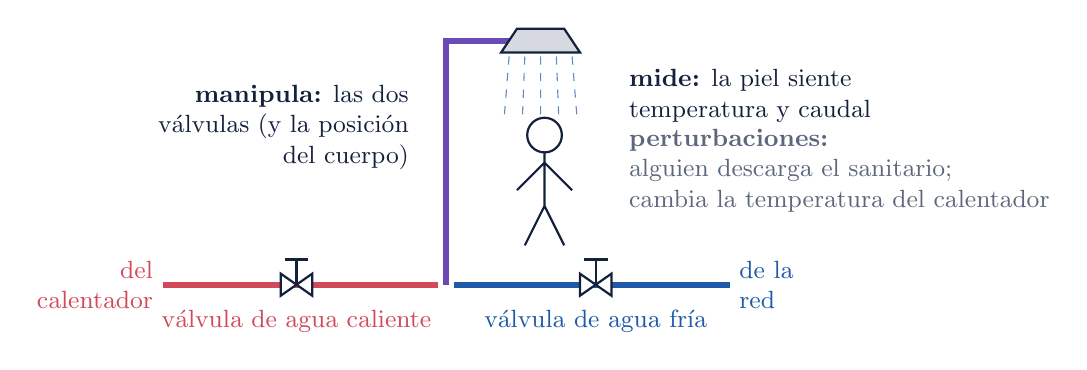
\begin{tikzpicture}[font=\footnotesize,
  valvula/.pic={\draw[thick,ctrlnoche,fill=white] (-0.2,-0.14)--(0.2,0.14)--(0.2,-0.14)--(-0.2,0.14)--cycle; \draw[thick,ctrlnoche] (0,0)--(0,0.32) (-0.15,0.32)--(0.15,0.32);}]
  % tuberías
  \draw[line width=2.2pt,ctrlcoral] (-3.6,0)--(-0.1,0);
  \draw[line width=2.2pt,ctrlazul] (3.6,0)--(0.1,0);
  \draw[line width=2.2pt,ctrlvioleta] (0,0)--(0,3.1)--(1.1,3.1);
  \pic at (-1.9,0) {valvula}; \pic at (1.9,0) {valvula};
  \node[below=3pt,text=ctrlcoral] at (-1.9,-0.1) {válvula de agua caliente};
  \node[below=3pt,text=ctrlazul] at (1.9,-0.1) {válvula de agua fría};
  \node[left,text=ctrlcoral,align=right] at (-3.6,0) {del\\calentador};
  \node[right,text=ctrlazul,align=left] at (3.6,0) {de la\\red};
  % regadera
  \draw[thick,ctrlnoche,fill=ctrlgris!25] (0.9,3.25)--(1.5,3.25)--(1.7,2.95)--(0.7,2.95)--cycle;
  \foreach \x in {0.8,1.0,1.2,1.4,1.6}{\draw[ctrlazul!70,dashed] (\x,2.9)--(\x+0.15*\x-0.18,2.15);}
  % persona
  \begin{scope}[xshift=1.25cm,yshift=0.35cm,thick,ctrlnoche]
    \draw (0,1.55) circle (0.22);
    \draw (0,1.33)--(0,0.65) (0,1.2)--(-0.35,0.85) (0,1.2)--(0.35,0.85) (0,0.65)--(-0.25,0.15) (0,0.65)--(0.25,0.15);
  \end{scope}
  % anotaciones
  \node[align=left,anchor=west,text=ctrlnoche] at (2.2,2.4) {\textbf{mide:} la piel siente\\temperatura y caudal};
  \node[align=left,anchor=west,text=ctrlgris] at (2.2,1.45) {\textbf{perturbaciones:}\\alguien descarga el sanitario;\\cambia la temperatura del calentador};
  \node[align=right,anchor=east,text=ctrlnoche] at (-0.35,2.0) {\textbf{manipula:} las dos\\válvulas (y la posición\\del cuerpo)};
\end{tikzpicture}
\end{document}
